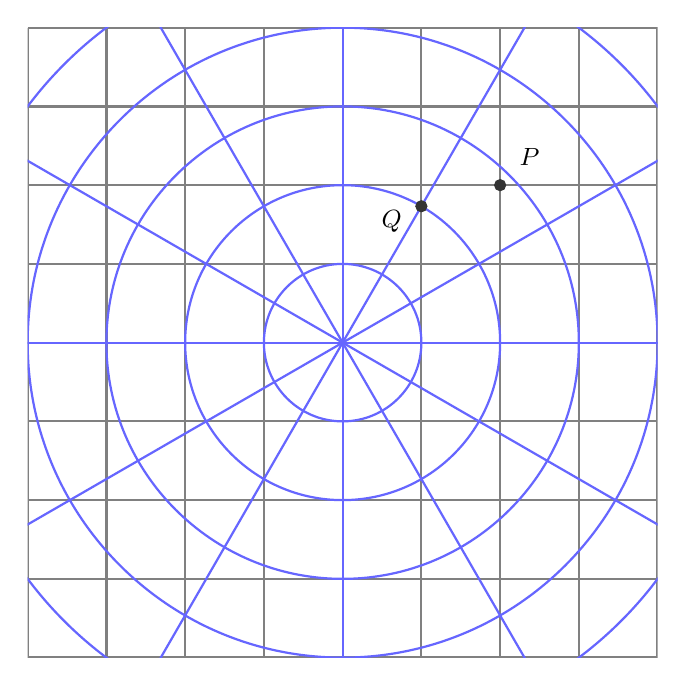
\begin{tikzpicture}
    \clip (-4,-4) rectangle (4,4);
    \draw[step=1cm,gray,thick] (-4,-4) grid (4,4);
    \foreach \i in {1,...,6}{
        \draw[blue!60,thick] (0,0) circle (\i);
    }
    \foreach \i in {0,...,12}{
        \draw[blue!60,thick] (0,0) -- (canvas polar cs:angle=\i*30,radius=5cm);
    }
    \filldraw[black!80] (2,2) circle (2pt);
    \node[label={[black, font=\small]45:$P$}] at (2,2) {};
    \filldraw[black!80] (canvas polar cs:angle=60,radius=2cm) circle (2pt);
    \node[label={[below left, black, font=\small]150:$Q$}] at (canvas polar cs:angle=60,radius=2cm) {};
\end{tikzpicture}